\documentclass[main]{subfiles}
\begin{document}
%@@@@@@@@@@@@@@@@@@@@@@@@@@@@@@
% summarizes lecture 4
% author: David Bontrager

\section{Current source}
%David
This is another iteration of ``we call this a circuit but really it is simply what transistors do.'' In this case, $V_s$, $V_d$, and $V_g$ are set to constant values and $I_{ds}$ is our output. In practice, we tie $V_s$ to ground, put $V_g$ at some value less than 0.7V (to keep it subthreshold), and $V_d$ is put above 100mv to keep it in saturation. If we use a long transistor we can ignore Early voltage effects.\\ \\
Technically this is a current \emph{sink}, not a current \emph{source} because the current is pulled into the drain from above\footnote{``Above'' refers to ``closer to $V_{dd}$''}. To have a current source that will go higher in the circuit than whatever is consuming your current, you simply use a pFET instead of an nFET, tie the source to $V_{dd}$, and set gate voltage such that $V_g > V_{dd} - 0.7$. In either case the equation to calculate output current is by definition the subthreshold saturation current $I_{ds} = I_0 \exp ( (\kappa V_g - V_s)/U_T )$.
%------Diode-connected transistor-------
\begin{figure}[ht]
 \centering
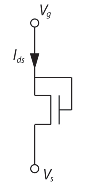
\includegraphics[natwidth=185,natheight=375]{figs/nme_diodeConn_transistor.pdf}
\caption{Diode-connected nFET \label{diodeConn}}
\end{figure}
\end{document}